\documentclass[12pt, letterpaper]{article}
\usepackage[utf8]{inputenc}
\usepackage{authoraftertitle}

% bibliography
\usepackage[style=authoryear,sorting=none,backend=biber]{biblatex}
\addbibresource{Report Bibliography.bib}

% images
\usepackage{graphicx}
\graphicspath{{..}}

% listing and its styles
\usepackage{lmodern}
\usepackage{amsmath}
\usepackage{xcolor}
\usepackage{listings}
\lstset{
  basicstyle=\ttfamily,
  columns=fullflexible,
  frame=single,
  breaklines=true,
  postbreak=\mbox{\textcolor{red}{$\hookrightarrow$}\space},
}

% Document metadata
\title{csar: Query-driven Code Search and Refactoring Framework}
\author{Deniz Ozmus}
\date{December 2017}

\def \supervisor {Michael Tautschnig}

% We load hyperref here as a hacky fix to the tableofcontents not rendering
\PassOptionsToPackage{hyphens}{url}
\usepackage{hyperref}

% Custom url line breaking
\renewcommand{\UrlBreaks}{\do\:\do\.\do\/\do\_\do\-\do\a\do\b\do\c\do\d\do\e\do\f\do\g\do\h\do\i\do\j\do\k\do\l
\do\m\do\n\do\o\do\p\do\q\do\r\do\s\do\t\do\u\do\v\do\w\do\x\do\y\do\z\do\A\do\B\do\C\do\D\do\E\do\F
\do\G\do\H\do\I\do\J\do\K\do\L\do\M\do\N\do\O\do\P\do\Q\do\R\do\S\do\T\do\U\do\V\do\W\do\X\do\Y\do\Z}

% Document
\begin{document}

% DEBUG: Make sure all references show up at the end, whether used or not
\nocite{*}

% Title page
\begin{titlepage}
  \centering
  {\Large \MyTitle\par}
  \vspace{3cm}
  {\MyAuthor\par}
  \vspace{0.5cm}
  {\itshape Supervised by }{ \supervisor\par}
  \vspace{13cm}
  {\today\par}
\end{titlepage}

% Abstract
\begin{abstract}
  Software developers frequently search code.
  Semantics-based code searching is a context sensitive variant of code searching.
  There is currently a lack of semantics-based code search tools and furthermore no semantics-based, integrated code search and refactor tool.
  This paper will detail the creation of the csar (code search and refactor) tool, which aims to be versatile, query-driven, semantics-based and language-agnostic.
  It will cover its aims, the pre-requisite knowledge to understand this paper, scope (primary, secondary, non-functional and selected), context, design (with a running example), implementation, testing, and analysis.
\end{abstract}
\newpage

% Table of contents
\tableofcontents
\newpage

% Introduction
\section{Introduction}
The problem this paper will detail the creation of the csar tool.
This introduction will explain the aims, scope and the pre-requisite knowledge required to understand this paper.

\subsection{Aims}
csar aims to be a unified framework for code searching and refactoring whose users are developers.
It will take as input descriptions of searches and corresponding refactors in a newly devised query language called the csar query language.
This results in a versatile and descriptive framework, which can target any programming language without the users needing to know the specifics.

Furthermore, csar aims to be flexible code-wise, hence most of its API will be publicly exposed and documented.
Users of csar will be able to extend csar, or embed csar into complex build processes and other applications.

For example, suppose a user wants to be able to move methods matching a certain signature.
They should be able to subclass an interface describing how to perform a refactor, and implement such functionality.
Then they will recompile and rebuild csar, and then use it.

For example, suppose a user wants to run csar from within a build script.
The output they retrieve should be in a format which suits their needs.
Furthermore, csar's exit codes and related behaviours should be well documented.

\subsection{Scope}
We will define csar in terms of its requirements, these are categorised as primary requirements (necessary functionality), secondary requirements (unnecessary but useful functionality), and non-functional requirements.
The final requirements it will have are described in the Scope subsection.

\subsection{Primary Requirements}
\begin{itemize}
  \item Use guide - a small document describing how to use the implemented functionality of csar.
  \item Query-driven - csar should operate on inputs in query form.
  \item Source code parsing - csar should be able to parse source code, otherwise it cannot search or refactor them with the necessary amount of flexibility.
  \item Searching - csar should be able to search source code.
  \item Custom search domains - the user should be able to specify what files to search within the input query.
  \item Refactoring - csar should be able to refactor the source base being operated on.
  \item Language-agnosticism - csar should be designed to be language-agnostic, such that it can operate on any language if it is implemented in a simple way.
\end{itemize}

\subsection{Secondary Requirements}
These requirements are non-essential, but may be addressed if there is sufficient time, or if priorities shift.
The benefits and implementation details of each will be outlined.

\subsubsection{Indexing parsed project source code}
In many cases csar may act on the same project code, perhaps with some differences.
We could make csar faster by taking this into account.
We would index parsed project code and only re-parse them if they have changed.

We have two storage approaches we can take:
\begin{enumerate}
  \item Storage Approach: Flat Files\newline
  Either map the files to a parallel hierarchy in `.csar` which contains their parsed outputs, or, store them all in the same folder where their file names are the hashes of the input files.
  The second approach may cause problems if hash collisions occur, thus an appropriate hashing algorithm must be used.
  The last modified dates of the source code and their parsed code can be used to determine which files require updating.
  \item Storage Approach: Database (i.e. SQLite)\newline
  Store a `(Path, LastModified, ParsedCode)` relation in the database, preferably in a `.csar` directory.
  Note: `LastModified` is a date, which is the last time that file was modified, as of when it was parsed.
  We can use this to determine which files need updating.
\end{enumerate}

It is important to note that using the last modified dates of files can be error-prone, since they can be spoofed, but it would offer no advantage to an attacker.

\subsubsection{Supporting Mercurial (hg)/Subversion (svn) repositories}
In rare cases csar may be used on a project using outdated version control systems, using them to narrow the search domain will be useful to the developer and make csar faster.
This would be done analogously to the git implementation, but the program arguments we use when invoking their binaries will be different.
Some possibilities are listed below:
\begin{itemize}
  \item Hg: 'hg status --all`
  \item Svn: `svn list -R' or `svn status'
\end{itemize}

\subsubsection{IntelliJ IDEA Integration}
We may want to integrate csar into the IntelliJ IDEA IDE such that if a user of csar uses this IDE, they can use csar from within it. 
csar can be integrated into it in one of two ways:
\begin{itemize}
  \item Internally - csar can be implemented as an alternative to IDEA's structural search,
  this would enable it to carry out the following tasks:
  identifier usage finding, overridden method finding, type hierarchy resolving, refactoring, and semantics-based searching.
  This requires placing our code in \href{https://github.com/JetBrains/intellij-community/tree/master/platform/structuralsearch/source/com/intellij/structuralsearch}{platform/structuralsearch/...} and creating adapters to enable our code to provide the same interface as the current IDEA ones, to ensure maximum compatibility.
  \item As a Plugin - csar can be implemented as a third-party plugin which introduces a new query field.
  This field would allow users to type csar queries and then execute them, displaying the results in a standard IDEA result window.
\end{itemize}

\subsection{Non-functional Requirements}
\begin{itemize}
  \item Documentation - csar will be accompanied by four pieces of documentation: the report (design and implementation details), javadocs (component-level details), readme (how to run csar), and the user guide (how to use csar).
  \item Efficiency - the implementation will maximize the usage of algorithms which run in polynomial time.
  It will also be benchmarked against a large input, to highlight deficiencies.
  \item Extensibility - csar will be open source, will be language-agnostic so that users can easily implement support for their language of choice, will expose a public API with great usage of interfaces, and will thoroughly utilize dependency injection to allow third-party developers to customize its behaviour.
  \item Interoperability - csar will have a user guide explaining how to invoke it from other applications and will support flexible output formats.
  \item Open source
  \item Portable - csar will be written in Java (version 8) which is a cross-platform framework.
  Java 8 runs on platforms including recent versions of Windows, Mac OS X, and various Linux distributions \autocite{javasysreqs}.
  \item Quality/Reliability - csar will be well designed and make appropriate use of configuration management and unit testing to detect bugs early in the software development life cycle.
  csar will also make use of well-tested and maintained libraries and platforms where possible (within reason).
  If necessary, contributions to third-party libraries will also be made to ensure high quality dependencies.
  \item Scalability - csar will be multi-threaded, hence in general the more cores a user has available the faster it will be.
  Caching will also be used where appropriate so that larger input projects run in reasonable time.
  \item Testability - csar will be designed to make testing easy (e.g. heavy use of dependency injection).
  Test-Driven Development will also be used where appropriate, to ensure each component of csar works as intended.
\end{itemize}

\subsection{Scope}
This project has strict deadlines, so not every feature will be fully implemented.
The selected requirements (scope) of this project will be detailed in this section.

The query language will have two versions: 1.x.x (implemented) and $ \geq $ 2.x.x (potential improvements).
The implemented version will formally define the scope of the query language in the implementation, and the potential improvements version will define a more exhaustive schema.
My goal is not to develop an exhaustive query language which can express any language element in any language since it would take very long (it would constitute an entire project itself), hence $ \geq $ 2.x.x will be more exhaustive than 1.x.x but not the ultimate query language.

Parsing of java source code (Java 8) will be supported.
csar will be designed such that other programming languages can easily be integrated into it in the future.
A developer will need to write a plugin for each programming language they wish to use, analogously to how the java plugin will be written.
This will include the implementation of a language parser, post-processors, searcher, and refactorer.

Searching will be implemented to only work on methods (finding their definitions and usages) for now.
To implement it for the other language elements described in the query language would be as simple as copy-pasting the code for method searching and changing the types and getters involved.
However, this would be a greatly time consuming and tedious task.
It is also possible that further complications may arise which may need to be addressed in the form of post-processors for the programming languages, this is especially true for dynamic programming languages.

It will also support narrowing the search domain by a `.gitignore' file for directories which are git repositories, and by a custom `.csarignore' file.
Support for other version control systems are a backlog task and may not be fulfilled, but will follow trivially from the git implementation.
The git implementation will require calling the git binary with a specific argument and reading the output, which will reveal which files it is currently tracking.

Refactoring is very complicated and time consuming, so we will only consider two operations.
The first is changing method parameters, this involves resolving all usages of the method in question (in various contexts), modifying the method calls and its definition and ensuring no naming collisions occur.
The second is renaming methods, this should follow from changing method parameters, since if we resolve all method usages we should be able to simply rename them all and ensure no naming collisions occur.
Renaming is a very common activity for our users (programmers) and hence very valuable to include \autocite{murphy2012we}.

The program output could technically support thousands of formats, but for simplicity it will only support two: plain text and JSON.
If alternatives are required, a third-party developer will be able to easily add their own result formatter.

Efficiency will mainly be addressed by introducing multi-threading and caching where possible.
Specific algorithms to be used are currently unknown, but may become available as the details of the implementation are gradually addressed.

\subsection{Pre-requisite Knowledge}
``Refactoring is the process of changing the structure of software without changing its behavior." \autocite{murphy2012we} The aim of this is to improve the maintainability and readability of the code.

``Semantics-based search seeks to improve search accuracy by understanding the searcher's intent and the contextual meaning of terms as they appear in the searchable dataspace, whether on the Web or within a closed system, to generate more relevant results." \autocite{wikipediasemanticsearch} Henceforth, this is what is meant by `code search' or `search'.

Searching is important because it increases developer productivity by enabling reuse and this accounts for a significant portion of a developer's activity \autocite{reiss2009semantics,stolee2014solving}.

There have been attempts to solve searching which have failed including:
\begin{itemize}
  \item CodeGenie which used user-defined test cases to build search queries;
  \item Various works using keywords from comments and variable names;
  \item Assieme, Sorcerer, and Codifier which incorporate program code semantics \autocite{reiss2009semantics};
  \item AutoQuery (see \nameref{sec:AutoQuery}).
\end{itemize}

The reasons for their failures include: trying to do too much or too little, requiring too much user input, and yielding irrelevant search results \autocite{reiss2009semantics,stolee2014solving}.

Automated refactoring increases developer productivity by attempting to automate common tasks, and this accounts for a significant portion of a developer's activity \autocite{mens2004survey,murphy2012we}.

There have been attempts to solve automated refactoring which have failed including:
\begin{itemize}
  \item IntelliJ IDEA - this is an IDE with integrated automated refactoring.
  \item Netbeans - this is an IDE with integrated automated refactoring.
  \item Eclipse - this is an IDE with integrated automated refactoring.
\end{itemize}

The reasons for their failures includes: the degree of automation, reliability, configurability and openness, coverage, scalability, and language independence. \autocite{mens2004survey} Furthermore, we can conclude that existing tools have failed because they are underused \autocite{murphy2012we}.

Searching and refactoring are both hard to implement because optimally they should be language-agnostic \autocite{mens2004survey,reiss2009semantics}, which results in a trade-off between expressiveness and how language-agnostic you want the implementation to be.

csar parses source code to operate on it, ``parsing, syntax analysis or syntactic analysis is the process of analysing a string of symbols, either in natural language or in computer languages, conforming to the rules of a formal grammar." \autocite{wikipediaparsing}

csar frequently uses the visitor design pattern to iterate over the elements of a source file.
``The visitor design pattern is a way of separating an algorithm from an object structure on which it operates." \autocite{wikipediavisitorpattern}

csar uses ANTLR, which is a parser-generator, which in conjunction with appropriate grammars, will recognize and parse languages.

``A compiler-compiler (also known as a parser-generator) is a programming tool that creates a parser, interpreter, or compiler from some form of formal description of a language and machine. The input may be a text file containing the grammar written in BNF or EBNF that defines the syntax of a programming language, and whose generated output is some source code of the parser for the programming language, although other definitions exist." \autocite{wikipediacompilercompiler}

% Design
\section{Design}

The design of csar will be described in terms of the execution environment, an overview of what it does, a running example corresponding to this overview, and a high-level (component-wise) structure.

\subsection{Execution Environment}
csar will work on any recent, mainstream variant of Windows, Mac, or Linux, which has Java 8 (or above) installed and has sufficient memory.
The csar binaries should be placed in the same folder that you wish to conduct your search in, alongside your `.csarignore' file if you have one.

\subsection{Overview}
Firstly, a chosen csar frontend containing a main method is invoked by the JVM.
This frontend should query the user for some input defining what the user wants csar to do.
The provided `csar-cli' takes the input as command-line arguments which includes a non-optional csar query.

A csar query is a query-based description of what csar should do, this must include a searching action but not necessarily a refactoring action.

Then, the frontend parses these arguments and then calls upon the `csar-api' to carry out the work it has determined the user wants.
The `csar-api' carries out the following tasks in order:
\begin{itemize}
  \item Load plugins.
  \item Parse the csar query.
  \item Parses the project code.
  \item Post-processes the project code.
  \item Searches the project code.
  \item Refactors the project code (if applicable).
\end{itemize}
If an error occurs during any one of these tasks csar will respond appropriately, which may be modified through subclassing.
By default, in `csar-cli' csar will terminate with an appropriate error code.

Then, the frontend reads the appropriate results (refactoring results if available, otherwise the search results), and displays them in a suitable manner for the user.
Finally, `csar-cli' will terminate.

\subsection{Running Example}
Suppose we invoke `csar-cli' from the command-line with the following command: `java -jar csar.jar SELECT method:def:parse REFACTOR RENAME:parse2 -t 1'.
Furthermore, suppose our project has the following code files in the directory `/project/' alongside the csar binaries:

`Main.java':
\begin{lstlisting}[language=Java]
public class Main extends Parser {

  public static void main(String[] args) {
    new Main().run();
  }

  public void run() {
    parse();
  }
}
\end{lstlisting}

`Parser.java':
\begin{lstlisting}[language=Java]
public class Parser {

  public void parse() {
    // ...
  }
}
\end{lstlisting}

Firstly, `csar-cli' will parse these command-line arguments to instantiate a corresponding instance of `Csar', and the thread count will be set to 1.
The directory is not home to a supported version control and does not have a `.csarignore' file so no filtering of its contents will be applied.

Secondly, csar query language will be parsed.

Thirdly, each loaded language plugin will perform the following:
\begin{itemize}
  \item The project code will be parsed (on a single thread).
  \item The project code will be post-processed.
  \item The search will be performed.
  In this case method definitions which have the name `parse' will be stored in a search results list.
  We will have the following search results:
  \begin{lstlisting}
  (path='/project/Parser.java', lineNumber=3, codeFragment='  public void parse() {')
  \end{lstlisting}

  These results will be formatted and then printed as follows:
  \begin{lstlisting}
  Search Results:
  /project/Parser.java:3 - '  public void parse() {'
  \end{lstlisting}
  \item The refactor will be performed.
  In this case all definitions and corresponding usages (these are graphed in the code post-processing) in the search results list will have their identifier names changed to `parse2'.
  These changes will then be written to the relevant source code files.
  
  We will end up with the following code files:

  `Main.java':
  \begin{lstlisting}[language=Java]
  public class Main extends Parser {
  
    public static void main(String[] args) {
      new Main().run();
    }
  
    public void run() {
      parse2();
    }
  }
  \end{lstlisting}
  
  `Parser.java':
  \begin{lstlisting}[language=Java]
  public class Parser {
  
    public void parse2() {
      // ...
    }
  }
  \end{lstlisting}
  
  Furthermore, we will have the following refactor results:
  \begin{lstlisting}
  (path='/project/Main.java', lineNumber=8, codeFragment='    parse2();')
  (path='/project/Parser.java', lineNumber=3, codeFragment='  public void parse2() {')
  \end{lstlisting}
\end{itemize}

These results will be formatted in `csar-cli' and then printed as follows:
\begin{lstlisting}
Refactor Results:
/project/Main.java:8 - '    parse2();'
/project/Parser.java:3 - '  public void parse2() {'
\end{lstlisting}

Finally, `csar-cli' will terminate.

\subsection{High-level Structure}
This is a component-wise description of the structure of Csar.

\subsubsection{Component Overview}
\begin{figure}[!hb]
  \centering
  \caption{High-level Structure}
  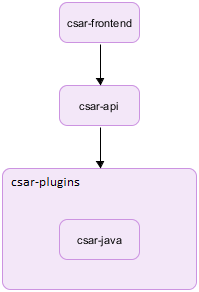
\includegraphics{figure-1}
\end{figure}

A command-line interface `csar-frontend' for csar is provided called `csar-cli', however a user can write their own.

The `csar-api' defines the csar query, csar plugins (using PF4J), and various utilities.
It does not specify language-specific implementation details.

The language-specific details are specified in plugins (see: `plugins').
These behaviours are: code parsing, post-processing, searching, and refactoring.

Plugins exhibit a few behaviours of note:
\begin{itemize}
  \item Plugins are not executed concurrently but interleaving during the same step of csar process may occur, i.e. all plugins may be told to parse one by one, then to post-process one by one, etc.
  \item Plugins have unrestricted access to the host machine.
  \item All plugins have access to all project files, thus it is possible for two plugins to modify the same file.
\end{itemize}

To create a plugin for csar the following must be done:
\begin{itemize}
  \item Create a new JVM project which has as dependency: `csar-api'.
  \item Create a class which implements CsarPlugin from `csar-api'.
  This should have a public 0-arguments constructor, and should implement the behaviour defined by the interface: parsing, processing, searching, and refactoring.
  You should make sure to delegate any errors to the attached error listeners.
  This is where the language-specific work occurs.
  Example:
  \begin{lstlisting}[language=Java]
  package org.qmul.csar;

  import org.qmul.csar.plugin.CsarPlugin;
  import org.qmul.csar.query.CsarQuery;
  import org.qmul.csar.result.Result;

  import java.nio.file.Path;
  import java.util.List;

  /**
    * The java language csar plugin.
    */
  public class CsarJavaPlugin implements CsarPlugin {

    @Override
    public void parse(Path projectDirectory, boolean narrowSearch, Path ignoreFile, int threadCount) {
      // parsing code...
    }

    @Override
    public void postprocess() {
      // post-processing code...
    }

    @Override
    public List<Result> search(CsarQuery csarQuery, int threadCount) {
      // searching code...
    }

    @Override
    public void addErrorListener(CsarErrorListener errorListener) {
      // add the error listener...
    }

    @Override
    public void removeErrorListener(CsarErrorListener errorListener) {
      // remove the error listener...
    }
  }
  \end{lstlisting}
\end{itemize}

To use the plugin with csar the following must be done:
\begin{itemize}
  \item Compile the project into JAR format place it in the current working directory.
  \item Define a resource for the JAR, which should go into the `META-INF/services' folder.
  The file's name should be `org.qmul.csar.plugin.CsarPlugin' and its content the name of your plugin.
  In our case this was `org.qmul.csar.CsarJavaPlugin'.
  \item Run the csar front-end jar, it should automatically detect and delegate tasks to your plugin.
\end{itemize}

\subsubsection{csar-cli}
csar-cli's command-line usage format has a non-optional search query, and is as follows:
\begin{lstlisting}
Usage: java -jar csar.jar [options] Search query
  Options:
    --threads, -t
      Thread count (default: 1)
    --log-level
      Log level (default: INFO)
      Possible Values (most restrictive to least): ERROR, WARN, INFO, DEBUG, TRACE
    --format, -f
      Output format (default: PlainText)
      Possible Values: PlainText, JSON
    --narrow-search
      Narrow search domain (default: true)
    --ignore-file
      Ignore file (default: .csarignore)
    --project-url, --url
      Print project URL
    --help, -h
      Print help information
\end{lstlisting}

These command-line arguments are stored in an instance of `CsarContext' using the JCommander library.
JCommander uses reflection to try to match the command-line arguments with fields in `CsarContext' using their configuration in their `@Parameter' annotations.
JCommander will also use the classes `Slf4jLevelConverter' and `ResultFormatterConverter' to convert the textual representations of log levels and result formatters respectively to instances.

Then, `CsarFactory' will use this instance of `CsarContext' to create a corresponding instance of `Csar'.
Furthermore, this `Csar' instance will have a default error listener attached to it which terminates the program with certain return codes depending on which fatal error occurs.
These return codes are follows:

\begin{tabular}{ l l }
  Exit Code & Description \\
  0 & Successful execution. \\
  1 & Error parsing CLI arguments. \\
  2 & Error parsing csar query. \\
  3 & Error parsing code files. \\
  4 & Error searching code files. \\
  5 & Error initializing csar. \\
  6 & Error post-processing code files. \\
  7 & Error formatting search results. \\
\end{tabular}

Then it will operate on the Csar instance performing the following tasks in order: initialize, parse query, parse code, post-process, search code and then refactor.
Once `Csar' has finished running, `csar-cli' will use the specified `ResultFormatter' to format these results, and then will print them.

It is important to note that, you could build your own frontend on top of `csar-cli' to create `Csar' instances using `CsarContext'.
This is useful because `CsarContext' is simple, has more configurable fields than exposed through the command-line interface, and also allows sub-classing.

\subsubsection{csar-api}
...
% TODO write about: Csar, error listener, plugin, lang, io, code, query, result, util

\subsubsection{csar-java}
...
% TODO write about: parsing, post-processing, search

% Implementation
\section{Implementation}
% TODO write about _how_ some classes from each component _exactly_ work

% Background Material
\section{Background Material}
\subsection{Related Academic Works}
\begin{itemize}
  \item \href{http://www.sciencedirect.com.ezproxy.library.qmul.ac.uk/science/article/pii/S1045926X16300970?_rdoc=1&_fmt=high&_origin=gateway&_docanchor=&md5=b8429449ccfc9c30159a5f9aeaa92ffb&ccp=y}{Ge X, Shepherd D, Damevski K \& Murphy-Hill E. (2016). Design and evaluation of a multi-recommendation system for local code search. \textit{International Journal of Computer Applications}. 138 (6). 9-13.}\newline
  This work is regarding plain-text code search in local projects and includes various ideas for optimisations.
  \item \href{https://link-springer-com.ezproxy.library.qmul.ac.uk/article/10.1007%2Fs10515-014-0170-2}{Wang S, Lo D \& Jiang L. (2016). AutoQuery: Automatic Construction of Dependency Queries for Code Search. \textit{Automated Software Engineering}. 23 (3). 393-425.}\newline
  This work is regarding dependence-based code searching.
  They have also devised a query language to make producing Program Dependency Graphs easier.
  \item \href{http://dl.acm.org.ezproxy.library.qmul.ac.uk/citation.cfm?id=2393612}{Shepherd D, Damevski K, Ropski B \& Fritz T. (2012). Sando: an extensible local code search framework. \textit{Proceedings of the ACM SIGSOFT 20th International Symposium on the foundations of software engineering}.}\newline
  This work is regarding an extensible plain-text code search in local projects.
\end{itemize}

There is also a lot of work on code search engines, ranking code samples and text matching, but these are mostly irrelevant to the development of csar.

\subsection{Related Programs}
\begin{itemize}
  \item \href{https://en.wikipedia.org/wiki/Grep}{grep}\newline
  A command-line utility for searching plain-text data against a regular expression.
  \item \href{https://beyondgrep.com/}{ack}\newline
  A command-line utility for searching plain-text data against a regular expression - essentially a better grep.
  \item \href{https://github.com/ggreer/the_silver_searcher}{ag (aka the silver searcher)}\newline
  A command-line utility for searching plain-text data against a regular expression - essentially a better ack.
\end{itemize}

\subsection{Query Language Analysis}
The following languages do not necessarily address my problem but they may influence the development of my own query language.

\subsubsection{AutoQuery}
\label{sec:AutoQuery}
Its queries are broken up into the following groups: program element types (variable, function, etc.) and identifier (if applicable), program element descriptions (contains, ofType, atLine, etc.), relation descriptions (depends on, etc.) and finally targets.
Each group can have 0 or more pieces of information within it, so it is descriptive.

Its language is unnatural (with respect to English) and is very rigid.
You can specify file, line number, types, and various elementary language elements (classes, methods, control flow).
It is not very expressive: it cannot represent try-catch blocks, anonymous methods/classes, and a long list of such constructs.

\subsubsection{AspectJ}
\href{https://eclipse.org/aspectj/doc/next/progguide/starting-aspectj.html}{AspectJ} has developed a language which it uses to address the problems presented by aspect-oriented programming.  

Their queries have a syntax that closely resembles that of Java. Examples below:
\begin{itemize}
  \item `call(void Point.setX(int)) || call(void Point.setY(int))'`'
  \item `call(void Figure.make*(..))'
  \item `call(public * Figure.* (..))
\end{itemize}

You can restrict the domain of queries with logical operators (and, or and not).
It has limited wildcards (`*', `..' which serves as `*' specially for method parameters, but it lacks `?').

You can define a query with an alias, which helps address the Don't Repeat Yourself principle, and thus verbosity.
I can also use this to provide coding standards verification (i.e. define queries and run them against the project, with matches corresponding errors in standards).
You can define method parameters as a type list or a named-type list which is flexible and expressive.

One issue is csar aims to be language-agnostic, so adopting a Java-like syntax will be unintuitive for non-Java programmers.

The syntax fails for dynamically-typed languages where types are not explicitly defined, so a method with signature: `my\_method(int)' would be invalid (or require additional processing to make work).
A solution to this is accepting variable name lists.

\subsubsection{Infer}
\href{https://github.com/facebook/infer}{Infer} has developed a language called \href{https://code.facebook.com/posts/277643589367408/}{AL} which it uses to define code templates corresponding to code stink. Example below:  

\begin{lstlisting}
DEFINE-CHECKER STRONG_DELEGATE_WARNING = {
    LET name_contains_delegate = declaration_has_name(REGEXP("[dD]elegate"));
    LET name_does_not_contain_queue = NOT declaration_has_name(REGEXP("[qQ]ueue"));

    SET report_when =
        WHEN
            name_contains_delegate
            AND name_does_not_contain_queue
            AND is_strong_property()
        HOLDS-IN-NODE ObjCPropertyDecl;

    SET message = "Property or ivar %decl_name% declared strong";
    SET suggestion = "In general delegates should be declared weak or assign";
};
\end{lstlisting}

It is very descriptive (allows compositions with `AND', `NOT', `WHEN' etc.) and intuitive (similar to SQL). You can define strings as regex patterns, this is a powerful feature.
The language is verbose and thus does not resonate with csar's competitors, which use single line queries.
However, declarations and response messages can be useful for creating complex tools with csar (i.e. code convention checks).

\subsection{Code References}
\begin{itemize}
  \item Ignore files syntax - \url{https://git-scm.com/docs/gitignore} and \url{https://github.com/EE/gitignore-to-glob/blob/master/lib/gitignore-to-glob.js}
  \item Test cases for ignore files - \url{https://www.atlassian.com/git/tutorials/gitignore}
  \item Git repository integration - \url{https://git-scm.com/docs/git-ls-files}
  \item Java 8 ANTLR Grammar - \href{https://github.com/antlr/grammars-v4/blob/02711067f82bed8e0c8dfd25e80f4f8ae2472abd/java8-pt/JavaLexer.g4}{Java 8 Lexer}, \href{https://github.com/antlr/grammars-v4/blob/02711067f82bed8e0c8dfd25e80f4f8ae2472abd/java8-pt/JavaParser.g4}{Java 8 Parser}, \href{https://github.com/antlr/grammars-v4/blob/02711067f82bed8e0c8dfd25e80f4f8ae2472abd/_grammar-test/src/test/java/TestJava8pt.java}{Java 8 Test} and \href{https://github.com/antlr/grammars-v4/blob/02711067f82bed8e0c8dfd25e80f4f8ae2472abd/java8-pt/examples/AllInOne8.java}{Java 8 Test Input}
  \item `JAVA\_LETTER' rule in `CsarLexer' - \url{https://github.com/antlr/grammars-v4/blob/master/java8/Java8.g4}
  \item Using JCommander parameters in `CsarContext' - \url{http://jcommander.org/}
  \item ANTLR settings in `build.gradle' - \url{https://docs.gradle.org/4.0.1/userguide/antlr\_plugin.html\#sec:controlling\_the\_antlr\_generator\_process}
  \item JaCoCo in `build.gradle' - \url{http://www.jworks.nl/2013/06/03/jacoco-code-coverage-with-gradle/}
\end{itemize}

% Bibliography
\section{Bibliography}
\printbibliography[heading=none]

\end{document}
